\documentclass{resume}

\usepackage[left=0.75in,top=0.1in,right=0.75in,bottom=0.6in]{geometry}
\usepackage[utf8,latin1]{inputenc}
\usepackage{hyperref}
\usepackage{graphicx}
\usepackage{float}
\usepackage[absolute,overlay]{textpos}

\setlength{\TPHorizModule}{1mm}
\setlength{\TPVertModule}{1mm}
\graphicspath{ {./images/} }
\inputencoding{utf8}
%\inputencoding{latin1}

%\name{ Marlus Cadanus da Costa }
%\address{ Nilo Peçanha, 3803 \\ Curitiba, PR - 82120-440 - Brésil  }
%\address{ skype: marluscadanus \\ www.linkedin.com/in/marluscadanus \\ marluscadanus@gmail.com }

%\def\nameskip{\bigskip}
%\def\sectionskip{\medskip}

\begin{document}

 \begin{textblock}{20}(171,10)
    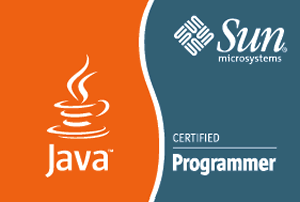
\includegraphics{java-certified-programmer}
 \end{textblock}

 \begin{textblock}{20}(171,30)
    
\includegraphics{java-certified-web}
 \end{textblock}

\begin{center}
  {\fontsize{16}{18} \bf Marlus Cadanus da Costa} \\\\
\end{center}
\begin{center}
  {\fontsize{12}{14} 3803, Rue Nilo Peçanha} \\ 
  {\fontsize{12}{14} Curitiba, Paraná - 82120-440 - Brésil} \\
  {\fontsize{12}{14} marluscadanus@gmail.com} \\
  {\fontsize{12}{14} skype: marluscadanus}
\end{center}

  \begin{rSection}{Sommaire}
  \end{rSection}

    \begin{itemize}
       \item Ingénieur de Logiciels détenant 9+ années d’expérience.
       \item Excellente connaissance de la programmation orientée objets avec C, C++ et Java.
       \item Riche expérience dans le domaine de développement des logiciels multiplateforme: Windows, Linux et Web.
       \item Capable d'apprendre et de s'adapter facilement.
       \item Français (avancé), Anglais (avancé) et Portugais (courant).
    \end{itemize}

  \begin{rSection}{Formation}
    {\bf Spécialisation en Informatique - Programmeur de Jeux Vidéo } \hfill {\em 2012} \\
    {PUC-PR, Curitiba - PR - Brésil} \\ 

    {\bf Baccalauréat en Informatique } \hfill {\em 2008} \\
    {Université Positivo, Curitiba - PR - Brésil}   
  \end{rSection}
  
  \begin{rSection}{Technologies Maitrisées}
    \begin{rSubsection}{}{}{}{}
      \item {\bf Concepts:} Design Patterns, OOP, UML, RUP, Scrum, Agile, SOA, BPM, TDD, BDD.
      \item {\bf Langages de programmation:} C, C++ et Java.
      \item {\bf Frameworks/APIs - Java EE:} Servlets, JSP, JSF, Spring, EJB, MDB, JMS, JPA, JDBC, Web Services (SOAP et REST).
      \item {\bf Frameworks/APIs/Utils - C:} C standard library, Sockets, p\_threads, CMake, GDB, Valgrind.
      \item {\bf Frameworks/APIs/Utils - C++:} Qt, Boost, STD, STL.
      \item {\bf Bases de données}: MySQL, PostgreSQL, Oracle et SQL-ANSI.
      \item {\bf Source Control Management Systems}: SVN, Git.
      \item {\bf Integrated Development Environments}: Qt Creator, XCode, Eclipse et Visual Studio.
      \item {\bf Modeling et Design}: Enterprise Architect, Bizagi, IBM Rational Software Architect.
    \end{rSubsection}
  \end{rSection}
  \begin{rSection}{Expérience Profissionnelle}

    \begin{rSubsection}{\fontsize{12}{14}\selectfont \bf Analyste et programmeur}{\fontsize{12}{14}\selectfont Fev. 2015 - Aujourd'hui}{\fontsize{12}{14}\selectfont Sascar}{}
    Sascar est une entreprise spécialisée dans la gestion de la flotte et de suivi des véhicules et du fret. Il est la seule entreprise au Brésil pour fonctionner sur une grande échelle avec les technologies GSM / GPS, satellite et radio fréquence. Ses solutions permettent une surveillance en temps réel des véhicules et des charges.\\\\
    \textit{Travaillé comme analyste et programmeur, participé à la conception et le développement d’applications client/serveur des systèmes de communication entre le hardware de localization et le front-end web.}

    \end{rSubsection}

      \begin{rSubsection}{\fontsize{9}{10}\selectfont Responsabilités:}{}{}{}
        \item Crée le design des systemes;
        \item Analysé, programmé et testé le code en C/C++ et Java;
        \item Effectué le déploiement, la gestion et le support de la solution;
      \end{rSubsection}

      \begin{rSubsection}{\fontsize{9}{10}\selectfont Projets significatifs:}{}{}{}
        \item Projet Kit Limpeza - Developpé un système pour tester des ports du hardware de localization des véhicules. Travaillé avec C/C++, sockets, p\_threads, Active MQ pour envoyer et recevoir des commandes aux equipments, et developpé le front-end avec Java, JSF, EJB, JPA et Web services.
      \end{rSubsection}

      {\fontsize{8}{9}\selectfont \textbf{Environnement technique:} Eclipse, QT Creator, C, C++, Sockets, p\_threads, , SVN, Java, JSF, EJB, JPA, Web Services, Active MQ, PostgreSQL.}\\

    \begin{rSubsection}{\fontsize{12}{14}\selectfont \bf Architecte et programmeur}{\fontsize{12}{14}\selectfont Déc. 2010 - Fev. 2015}{\fontsize{12}{14}\selectfont Winterlabs}{}
    La compagnie Winterlabs est une petite entrepise de development des systemes. Elle
détient de bureau à Curitiba au Brésil. \\\\
\textit{Travaillé comme architecte de solutions et programmeur, creé la conception, le développement et la recherche de meilleures solutions pour les applications d'entreprise.}
    \end{rSubsection}

      \begin{rSubsection}{\fontsize{9}{10}\selectfont Responsabilités:}{}{}{}
        \item Crée l’architecture des systemes;
        \item Analysé, programmé et testé le code en C/C++/Objective-C et Java;
        \item Effectué le déploiement, la gestion et le support de la solution;
        \item Évalué et testé nouvelles tecnologies;
      \end{rSubsection}

      \begin{rSubsection}{\fontsize{9}{10}\selectfont Projets significatifs:}{}{}{}
        \item Projet STAP - Mis en œuvre un simulateur de tir virtuel pour les forces armes du Bresil, développé le module qui contrôle la piste de tir utilisant \textbf{Java}, utilisé \textbf{C/C++} avec OpenGL pour rendre les scènes du stand de tir, utilisé \textbf{Jasper Reports} pour développer les rapports sur les sessions de tir et utilisé \textbf{MySQL} comme base de données.
        \item Projet SKY FIGHTERS - Développé un jeu de carte et stratégie pour \textbf{iOS} en utilisant \textbf{Objective-C} et cocos2d framework.
        \item Projet RESTA1 - Développé un jeux de plateau classique pour \textbf{iOS} en utilisant \textbf{Objective-C} et cocos2d framework.
      \end{rSubsection}

      {\fontsize{8}{9}\selectfont \textbf{Environnement technique:} Xcode, Objective-c, Eclipse, Java SE 1.6, Eclipse-RCP, SWT, QT Creator, C, Sockets, OpenCV, OpenGL, C++, SFML, GLSL, SVN, GIT, MySQL.}\\
    

    \begin{rSubsection}{\fontsize{12}{14}\selectfont \bf Analyste et programmeur}{\fontsize{12}{14}\selectfont Août 2008 - Déc. 2010}{\fontsize{12}{14}\selectfont GVT Telecom}{}
      GVT est une entreprise brésilienne avec des opérations depuis novembre 2000, qui fournit des services à large bande à l'échelle nationale avec de grande vitesse, la télévision par câble et convergente téléphonie fixe pour les clients résidentiels et des solutions d'affaires pour les entreprises.\\\\

      \textit{Impliqué dans toutes les étapes du cycle de développement de solutions de gestion des systèmes de télécommunications. Travaillé avec les intégrations de systèmes parmi toutes les équipes de l'entreprise à l'aide de SOA et BPM concepts.}
    
    \end{rSubsection}

      \begin{rSubsection}{\fontsize{9}{10}\selectfont Responsabilités:}{}{}{}
        \item Développé des modules pour les demandes des clients et mis à jour les web services dans un environnement SOA;
        \item Crée des modules pour les demandes des clients avec BPM;
        \item Analysé, programmé et testé le code en Java en utilisant JEE, EJB, JPA, JMS, MDB et JDBC;
        \item Effectué le déploiement, la gestion et le support de la solution;
        \item Crée et modifié les procédures stockées de la base de données
      \end{rSubsection}

      \begin{rSubsection}{\fontsize{9}{10}\selectfont Projets significatifs:}{}{}{}
        \item Projet "Nova Arquitetura OSS" - Développé une nouvelle interface de communication entre un neuf équipement ADSL et les systemes de l'entreprise. Travaillé avec Java, EJB, MDB, JPA et Web Services, utilisé Oracle 10g comme base de données et Oracle AQ.
        \item Projet "Serviços de Gerência" - Mis en œuvre un systeme web pour gerer les produits ADSL, en utilisant les technologies JAVA, JSP, JSTL et AJAX. Crée le business layer avec Spring, les rapports avec JasperReports et JFreeChart.
        \item Projet "Prevenção de fraudes" - Travaillé comme programmeur avec Java, Savvion BPM et Web Services pour développer une système de gestion des données des clients afin de prévenir les actions de fraude téléphonique.
      \end{rSubsection}
    
      {\fontsize{8}{9}\selectfont \textbf{Environnement technique:} Sparx Enterprise Architect, Eclipse, Java, JEE 1.5, Servlets, JSP, JSF, EJB (Session Beans et Entity Beans), JPA, MDB, JMS, Web Services, SOA, BPM, Savvion, ESB, Oracle Weblogic, AquaLogic Service Bus, Oracle AQ, Oracle 10g, PostgreSQL, Ant, Maven, Atlassian JIRA, SVN.} \\
    

    \begin{rSubsection}{\fontsize{12}{14}\selectfont Analyste et programmeur}{\fontsize{12}{14}\selectfont Janv. 2006 - Mai. 2008}{\fontsize{12}{14}\selectfont HSBC Banque}{}
    Fondée en 1865 et basée à Londres, HSBC est une des plus grandes organisations de services financiers et bancaire du monde.\\\\

    \textit{Travaillé sur plusieurs projets comme un analyste et programmeur. Développé des projets bancaires d'Internet et des systèmes de financement.}
    \end{rSubsection}
      \begin{rSubsection}{\fontsize{9}{10}\selectfont Responsabilités:}{}{}{}
        \item Développé des modules pour les services bancaires sur Internet;
        \item Analysé, programmé et testé le code en Java, Servlets, HTML, XML, XSLT et JavaScript;
        \item Effectué le déploiement, la gestion et le support de la solution;
        \item Crée et modifié les procédures stockées de la base de données;
        \item Développé des modules d'intégration bancaire entre Java (client/server) et Cobol CICS (mainframe)
      \end{rSubsection}

      \begin{rSubsection}{\fontsize{9}{10}\selectfont Projets significatifs:}{}{}{}
        \item Projet “HOB-PWS” - Développé un système pour les clients du HSBC sans compte bancaire payent leurs factures d'électricité et de l'eau sur Internet banking. Utilisé Java, XML, XSLT et HTML pour developpé le front-end et Java pour faire l'intégration avec Cobol CICS;
        \item Projet “CDCI”. Mis en œuvre un système de simulation de financement direct pour le client de détail. Fait le design de l’application utilisant le IBM RSA (Use cases diagrams, classes diagrams, sequence diagrams et activity diagrams). Développé dans le modèle MVC en utilisant Java, Eclipse-RCP et SWT;
        \item Projet “CNB-CED” - Creé un système de gestion des signatures de contrats de change pour les clients qui accèdent à l'Internet Banking du HSBC. Travaillé avec Java, SOA architecture, BPM et fait l'intégration avec le back-end Cobol CICS.
      \end{rSubsection}

      {\fontsize{8}{9}\selectfont \textbf{Environnement technique:} IBM Rational Software Architect, Eclipse, Eclipse-RCP, Java, C, SWT, Servlets, XML, XSL, JDBC, WSAD, Websphere 5.1, IBM MQSeries, SQL, Sybase, Oracle, CVS, SVN.}

  \end{rSection}

  \begin{rSection}{Certifications}
    {\bf Sun Certified Programmer for the Java 2 Platform 1.4}\\ 
    {Sun Microsystems, Inc.} \\

    {\bf Sun Certified Web Component Developer for the Java 2 Platform Enterprise Edition 1.5}\\ 
    {Sun Microsystems, Inc.} \\
  \end{rSection}

  \begin{rSection}{Cours Supplémentaires}
  \end{rSection}  

  \begin{itemize}
    \item 2006 - Object Oriented Analysis/UML
    \item 2005 - C PROGRAMMING
    \item 2005 - SQL ANSI
    \item 2004 - Workshop Java
    \item 2004 - Java Programming Language
  \end{itemize}

  
\end{document}
